\documentclass[../../main.tex]{subfiles}
\begin{document}

\subsection*{1.8}
Una particella di massa $m = 10^{-3}kg$ e carica $q_0 = -10^{-10} C$ è posta al centro di un anello di raggio R = 10 cm, su cui `e distribuita uni formemente la carica $q = 10-8 C$.
\\La particella viene spostata di un tratto $x_0 = 0.5 cm$ lungo l’asse e abbandonata. 
\\Dimostrare che la particella oscilla con moto armonico intorno all’origine e determinare il periodo T delle piccole oscillazioni e l’energia cinetica della particella quando passa per l’origine.
\\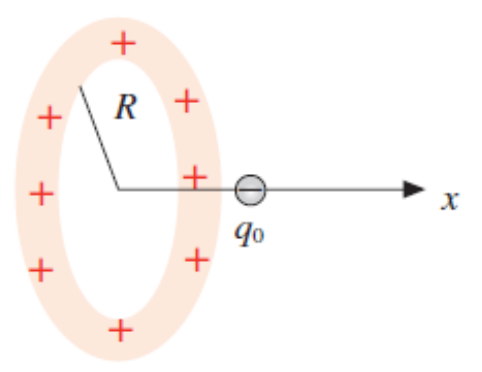
\includegraphics[scale=0.3]{e_1_8.png}
\subsubsection*{Formule utilizzate}
\subsubsection*{Soluzione}
Calcoliamo il campo per ogni infinitesimo di anello.
\\$dE_x(x)=\frac{1}{4\pi\epsilon_0}\frac{dq}{R^2+x^2}\frac{x}{\sqrt{R^2 + x^2}}$
\\$E_x = \int_{anello}dE_x = \frac{1}{4\pi\epsilon_0}\frac{1}{R^2+x^2}\frac{x}{\sqrt{R^2+x^2}}\int_{anello}dq = \frac{q}{4\pi\epsilon_0}\frac{x}{(R^2 +x^2)^{\frac{3}{2}}}$
\\Se $\left(\frac{x}{R}\right)^2 \ll 1 $
\\$\vec{E}(x) = \frac{1}{4\pi\epsilon_0}\frac{qx}{R^3}\vec{u_x}$
\\$\frac{m\ d^2x}{dt^2}+\frac{1}{4\pi\epsilon_0}\frac{q|q_0|}{R^3}x = 0$
\\$\omega = \sqrt{\frac{q|q_0|}{4\pi\epsilon_0mR^3}} = 0.0949\ rad/s $
\\con $T = 2\pi / \omega = 66,23\ s$
\\$E_k = \frac{1}{4\pi\epsilon_0}\frac{|q_0\ q|}{R^3}\int_0^{x_0}xdx = \frac{1}{4\pi\epsilon_0}\frac{|q_0\ q| x_0^2}{2R^3}=1.13 * 10^{-10}\ J$
\newpage

\end{document}